\section{TypeScript}
\label{sec:typescript}
TypeScript é uma linguagem de programação desenvolvida pela Microsoft em 2012 de código aberto. Por definição, consiste-se de um superconjunto do JavaScript, adicionando também tipagem estática a linguagem original \cite{Microsoft2023}.

Por tratar-se de superconjunto, tudo o que existe em sua linguagem “mãe” também está presente nesta linguagem, incrementada pelas novas suas funcionalidades, como por exemplo: tipos, orientação à objetos, \textit{decorators}, \textit{mixins}, módulos e \textit{namespaces} \cite{Goldberg2022}.Além disso, essa peculiaridade também faz com que todo código JavaScript também seja um código TypeScript minimamente válido, facilitando assim possíveis migrações de projetos.

Pela natureza do JavaScript de ser compilado \textit{just-in-time}, muitos erros frugais de desenvolvimento são percebidos apenas na hora da execução do código. Entretanto, pelo TypeScript ser estaticamente tipado, o paradigma de orientação a objetos é acentuadamente estimulado \cite{Goldberg2022}. Ao alinhar isso ao sistema de tipos da linguagem, erros de programação tornam-se evidentes muito brevemente, conforme exemplifica a  figura a seguir:

\begin{figure}[H]
    \centering
    \caption{Comparação de códigos TypeScript e JavaScript.}
    \label{fig:typescript}
    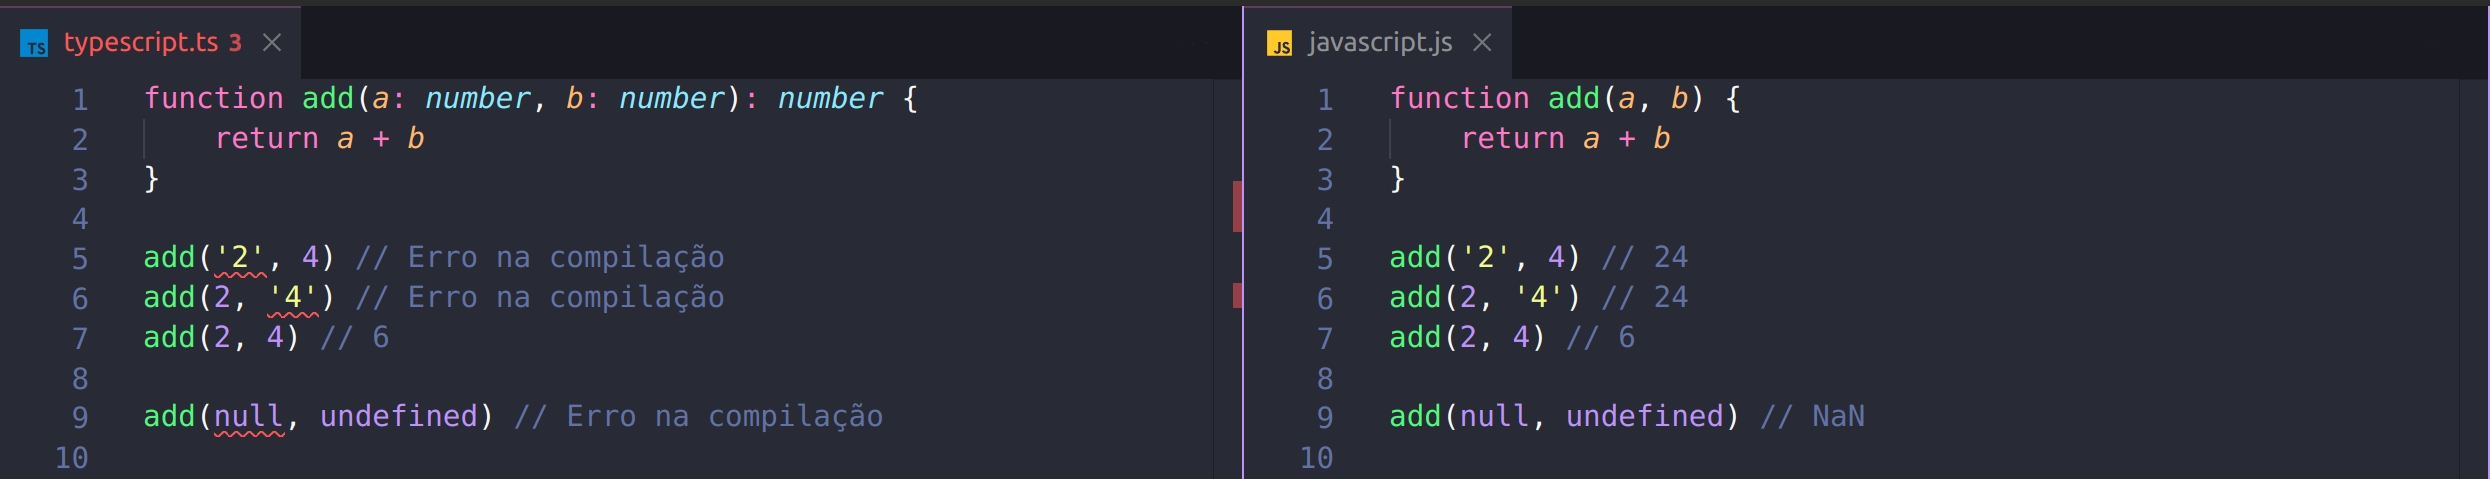
\includegraphics[width=1\textwidth]{data/figures/typescript-javascript.jpg}
    \fonte{Autor}
\end{figure}

Além de tudo, segundo \citeonline{Microsoft2023a}, a estrutura padrão do JavaScript acaba por não conseguir acompanhar o crescimento exponencial de tamanho, escopo e complexidade de suas novas aplicações, reduzindo a capacidade de escalabilidade da linguagem, problemática que é profundamente saciada pelas funcionalidades extras do TypeScript.

Por fim, pelos navegadores efetivamente darem suporte exclusivamente a códigos JavaScript, o TypeScript necessita ser pré-processado antes de ser empregado no \textit{client-side}, tornando sua linguagem “mãe” imprescindível à sua construção. Seu compilador padrão é o tsc, e outros agregadores mantidos pela comunidade (como o esbuild e o babel) podem ser utilizados a partir da necessidade específica de cada projeto \cite{Microsoft2023a}.

